\section{Discussion}

Furthermore, the distribution of respiratory viruses in this study was very different from that in our previous study. 

% why could we not detect so many bioaerosols

We detected fewer respiratory viruses in bioaerosol samples compared to our previous study\cite{Banholzer2023PLoSMed} (1~sample of adenovirus and 1~sample of rhinovirus in this study vs 10~samples of SARS-CoV-2 in the previous study), especially in relation to the number of positive saliva samples (50~samples in this study vs 21~in the previous study). Similarly, the number of viruses detected on the filters of the air cleaners was also lower in this study (4~positive samples in 160~swabs vs 8~positive samples in 80~swabs in the previous study). Importantly, there was a clear shift in the distribution of respiratory viruses in the current study compared to the previous study in 2022 during the SARS-CoV-2 Omicron variant. Whereas in 2022 we detected almost exclusively SARS-CoV-2 in human saliva, the most common respiratory viruses in 2023 were adenovirus, influenza~B, and rhinoviruses (only three SARS-CoV-2-positive samples). The shift in the pattern of respiratory viruses has been observed in other studies\cite{Nygaard2023Lancet,Sauteur2022EuroSurv}. 

% other reasons

Technical reasons for the differences in airborne detection are unlikely. The bioaerosol sampling devices and laboratory procedures were the same in both studies, and no technical problems were observed. Instead, airborne detection could have been influenced by environmental factors. Although temperature (overall between 19 and 25$^{\circ}$C) and relative humidity (overall between 25 and 50\%) were similar in both studies, the same levels may have different effects on the airborne survival of respiratory viruses. For example, airborne survival of rhinovirus and adenovirus increases with relative humidity, whereas the opposite relationship has been documented for influenza and SARS-CoV-2\cite{Tellier2009JTRSI,Ahlawat2020AAQR,Biryukov2020mS,Karim1985CJM,Davis1971AM}. A change in ventilation conditions could also have had a profound effect, but CO$_2$ levels were higher compared to the previous study (1,702$\pm$370\,ppm in this vs 1,064$\pm$232\,ppm in the previous study), suggesting that classrooms were not as well ventilated as during the COVID-19 pandemic. Although lower ventilation was partially offset by a greater reduction in aerosol and particle concentrations from air cleaners, the removal of particles by air cleaners may be slower than by natural ventilation.

% bioaerosol sampling in more depth

We speculate that the difference in airborne molecular detection of respiratory viruses between 2022 (pandemic) and 2023 (non-pandemic) is due to the different characteristics of the respiratory viruses. Differences in the physicochemical properties of virus-laden aerosols (\eg physical size, viral load, and infectivity), which influence the generation and survival of airborne viral RNA\cite{Wang2021,Sattar2016Book}, may facilitate the detection of SARS-CoV-2 in the air. The reason is that viral loads do often not exceed the detection limits of existing devices for bioaerosol sampling, which remains a challenge\cite{Wang2021,Belser2023PLOSPath,Bekking2019IORV,Mainelis2020AST}. For example, one study failed to detect any human rhinovirus in the exhaled breath of 16~HRV-infected subjects\cite{Fabian2011JAMPDD}. However, several studies showed that influenza\cite{Bischoff2013JID,Pan2017mSphere}, rhinovirus\cite{Myatt2004AJRCCM}, and adenovirus\cite{Nguyen2017OFID,Pan2017mSphere} can also be detected in airborne samples. Finally, the ability to detect pathogens in bioaerosols may be related to patient characteristics of the study participants. Several studies suggested an association between the generation of pathogenic aerosols and infectiousness\cite{Leung2020NatMed,Bischoff2013JID,Escombe2008PLoSMed}. Therefore, studies that include more infectious patients (intentionally or unintentionally) are likely to have a higher chance of detecting respiratory viruses in the air. 


\section{Comparison with previous study}\label{sec:comparison-prev-study}

% descriptive results

In a previous study\cite{Banholzer2023PLoSMed}, we estimated the effectiveness of mask wearing and air cleaners during the SARS-CoV-2 Omicron wave. \cref{fig:comparison} shows a comparison of the results. The distribution of respiratory infections is different (\cref{fig:comparison}a) because we almost exclusively detected SARS-CoV-2 in our previous study during the COVID-19 pandemic, as compared to a range of respiratory infections in this study during non-pandemic times. Although there were more positive saliva samples in this study, the number of respiratory infections detected in bioaerosols and on the HEPA-filters of the air cleaners was lower (\cref{fig:comparison}b).
The reductions in particle concentrations were larger and with lower uncertainty in this study (\cref{fig:comparison}c). The risk of infection tended to be lower with air cleaners in this study where air cleaners were analyzed using a cross-over design, but not in our previous study where air cleaners were installed only at the end of the study when most students had already been infected with SARS-Cov-2(\cref{fig:comparison}d).

% summary

To summarize, we found similar reductions in particle concentrations and a tendency for the relative risk of infection to be lower with air cleaners. To some extent, the differences between the two studies may be explained by different adjustments. While we could not adjust for ventilation in our previous study, the estimates in this study were adjusted for the daily air change rate, which correlated with the relative risk of infection (see \Cref{sec:detailed-molecular}). Furthermore, the distribution of respiratory viruses in this study was very different from that in our previous study and molecular airborne detection was lower.

\begin{figure}[!htpb]
    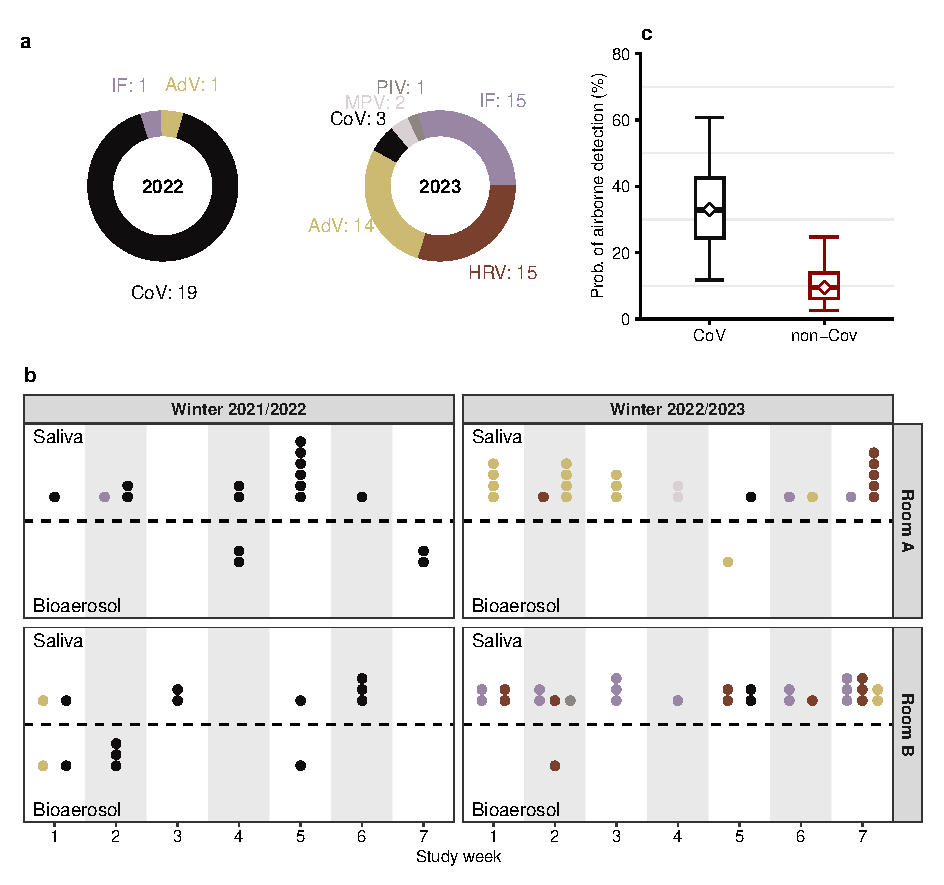
\includegraphics[width=\linewidth]{../../results/comparison.pdf} 
    \caption{\textbf{Comparison of the results between our previous study in 2022 during the COVID-19 pandemic (blue) and this study in 2023 during non-pandemic times (black).} \textbf{(a)}~Proportion of positive saliva samples by virus. Flu B: Influenza B, HRV: rhinovirus, AdV: adenovirus, CoV: SARS-CoV-2, MPV: metapneumovirus, PIV: parainfluenza virus. \textbf{(c)}~Estimated reduction in aerosol number and particle mass concentrations (CN in 1/cm$^3$) and particle mass concentration (PM for particles of sizes <1 to <10~$\mu$m, respectively in $\mu$gm$^{-3}$) with air cleaners (posterior mean as squares and 95\%-CrI as lines). \textbf{(d)}~Adjusted relative risk (ARR) of infection with air cleaners (posterior mean as squares and 95\%-CrI as lines).}
    \label{fig:comparison}
\end{figure}

% unlikely reasons for less airborne detection

Technical reasons for the differences in airborne detection are unlikely. The bioaerosol sampling devices and laboratory procedures were the same in both studies, and no technical problems were observed. Instead, airborne detection could have been influenced by environmental factors. Although temperature (overall between 19 and 25$^{\circ}$C) and relative humidity (overall between 25 and 50\%) were similar in both studies, the same levels may have different effects on the airborne survival of respiratory viruses. For example, airborne survival of rhinovirus and adenovirus increases with relative humidity, whereas the opposite relationship has been documented for influenza and SARS-CoV-2\cite{Tellier2009JTRSI,Ahlawat2020AAQR,Biryukov2020mS,Karim1985CJM,Davis1971AM}. A change in ventilation conditions could also have had a profound effect, but CO$_2$ levels were higher compared to the previous study (1,702$\pm$370\,ppm in this vs 1,064$\pm$232\,ppm in the previous study), suggesting that classrooms were not as well ventilated as during the COVID-19 pandemic. Although lower ventilation was partially offset by a greater reduction in aerosol and particle concentrations from air cleaners, the removal of particles by air cleaners may be slower than by natural ventilation. 

% likely reason for less airborne detection

More likely, SARS-CoV-2 may be easier to detect in the air due to physicochemical properties of virus-laden aerosols, so that its viral loads more often exceed the detection limits of existing devices for bioaerosol sampling,  which remains a challenge\cite{Wang2021,Belser2023PLOSPath,Bekking2019IORV,Mainelis2020AST}. For example, one study failed to detect any human rhinovirus in the exhaled breath of 16~HRV-infected subjects\cite{Fabian2011JAMPDD}. However, several studies showed that influenza\cite{Bischoff2013JID,Pan2017mSphere}, rhinovirus\cite{Myatt2004AJRCCM}, and adenovirus\cite{Nguyen2017OFID,Pan2017mSphere} can also be detected in airborne samples.